%!TEX root = ../../super_main.tex

\section{Customer Interaction}
\label{sec:customer_interaction}
To provide customers with a way of defining campaigns, and retrieving information from the system, a website have been created. This website is only available to customers, who may interact with the system in two ways, depending on their intent. Customers can, through a GUI, browse their previously created campaigns as well as create new ones. Alternatively, if customers wish to retrieve the gathered labeled training data, they may retrieve it in a JSON format which is interpretable by a computer. Both ways of interacting with the system will be described in this section. 
\\\\
The interface for the customer is meant to be some kind of expert system, where more explicit training in how to use the system might be necessary. This have been decided since we deem that the customers in need of snapshots will be willing to invest more effort into using the system in order to get the snapshots they desire. This means that some part of the system might somewhat less intuitive and requires some kind of tacit knowledge to be productive when using it. \tabref{tab:browser_routes} contains all routes that relates to the customer interaction of the system. This table effectively describes the full interface for the customers of the system since it is the complete list of routes they customer uses to interact with.

\begin{table}[!htbp]
    \centering
    \begin{tabular}{|l|l|} 
        \hline
        \textbf{Type} & \textbf{URL}                            \\ \hline 
        \mono{GET}    & \mono{campaigns}                        \\ \hline 
        \mono{POST}   & \mono{campaigns}                        \\ \hline 
        \mono{GET}    & \mono{campaigns/create}                 \\ \hline 
        \mono{GET}    & \mono{campaigns/\{campaign\}}           \\ \hline 
        \mono{GET}    & \mono{campaigns/\{campaign\}/snapshots} \\ \hline 
        \mono{GET}    & \mono{home}                             \\ \hline 
        \mono{POST}   & \mono{login}                            \\ \hline 
        \mono{GET}    & \mono{login}                            \\ \hline 
        \mono{GET}    & \mono{logout}                           \\ \hline 
        \mono{POST}   & \mono{password/email}                   \\ \hline 
        \mono{POST}   & \mono{password/reset}                   \\ \hline 
        \mono{GET}    & \mono{password/reset/\{token?\}}        \\ \hline 
        \mono{POST}   & \mono{register}                         \\ \hline 
        \mono{GET}    & \mono{register}                         \\ \hline 
    \end{tabular}
    \caption{The routes that the is used on the website.}
    \label{tab:browser_routes}
\end{table}
\FloatBarrier

Note that all screenshots of the customer UI containing an address bar includes the url \mono{https://dev.local.element67.dk:8000}, note that if you want to go visit the website as you read this you need to visit either \mono{https://prod.local.element67.dk:8000} (if you are on the AAU network) or \mono{https://prod.global.element67.dk:8000} (if you are not on the AAU network). Furthermore, mockups of this part of the system can be found in \appref{app:web_mockup}.
\\\\
When visiting the site, customers are presented with the page seen in \figref{fig:web_welcome}. Everybody, meaning both customers, participants, and people outside these categories, have access to this page, meaning that this welcome-page could be utilized to give the visitors more information regarding the system and the possibilities there lies within, which might lead to them becoming either customers or participants. 

% Welcome not logged in
\begin{figure}[!htbp]
\centering
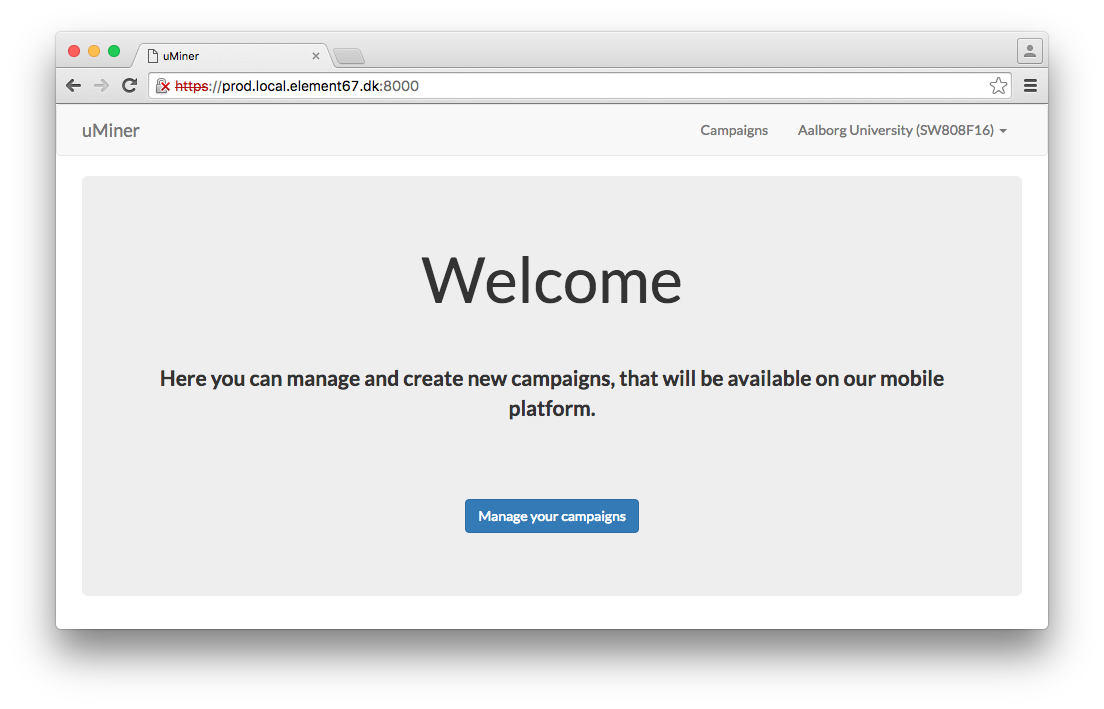
\includegraphics[width=\linewidth]{user_interfaces/web/web_welcome}
\caption{Welcome page.}
\label{fig:web_welcome}
\end{figure}
\FloatBarrier

\subsection{Registration and Logging In}

To gain access to the features of the website, customers must first log in. If the customer does not have a login, he can create one. The page for registration as well as the login page are similar to the ones of many other pages. When a user registers he is asked to provide a name, an email and a password. The name is used to show participants who created the different campaigns, allowing them to pick and choose which customers they wish to contribute data to. Please note that the same name can be shared by multiple accounts. This means that multiple accounts can be associated with \emph{Aalborg University}, for instance. Currently, everybody can register an account, but one could imagine that some level of verification might be required, so people cannot impersonate companies or persona. 

\todo[inline]{Jeg kunne forestille mig at det ville være beneficial at have conceptet om comapanies (customers) på web delen hvor flere users kan være tilknyttet det samme firma}

% % Register
% \begin{figure}[!htbp]
% \centering
% 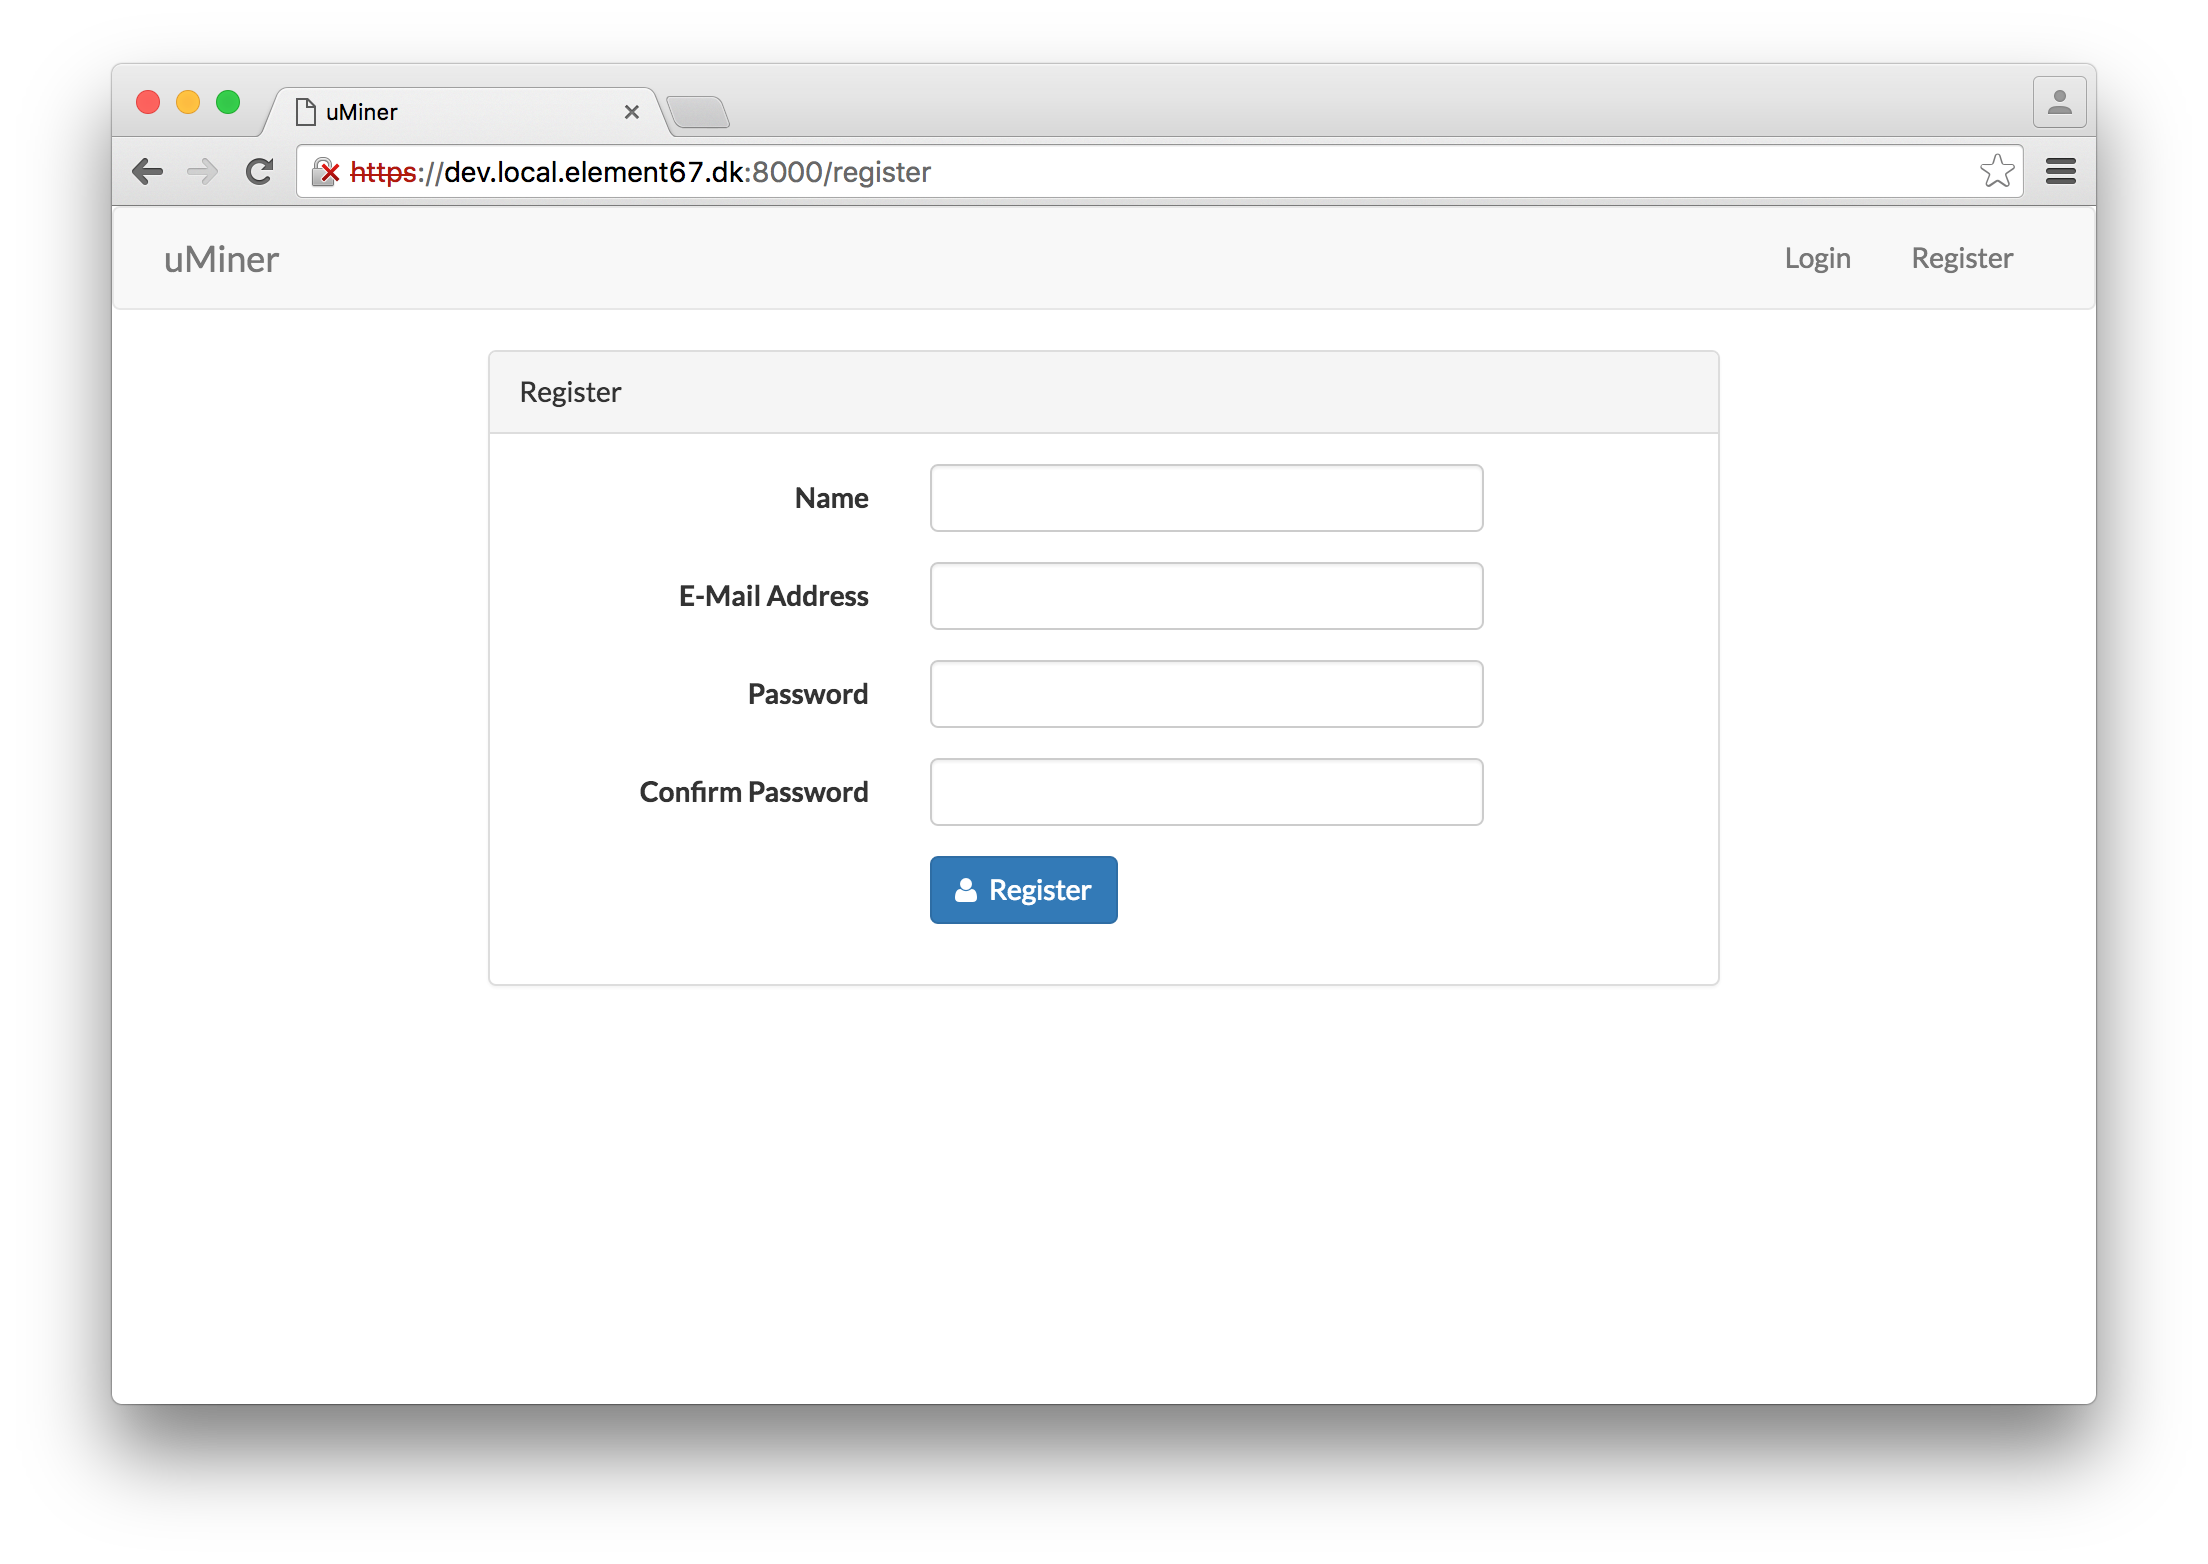
\includegraphics[width=\linewidth]{user_interfaces/web/web_register}
% \caption{Register page.}
% \label{fig:web_register}
% \end{figure}
% \FloatBarrier

% % Login
% \begin{figure}[!htbp]
% \centering
% 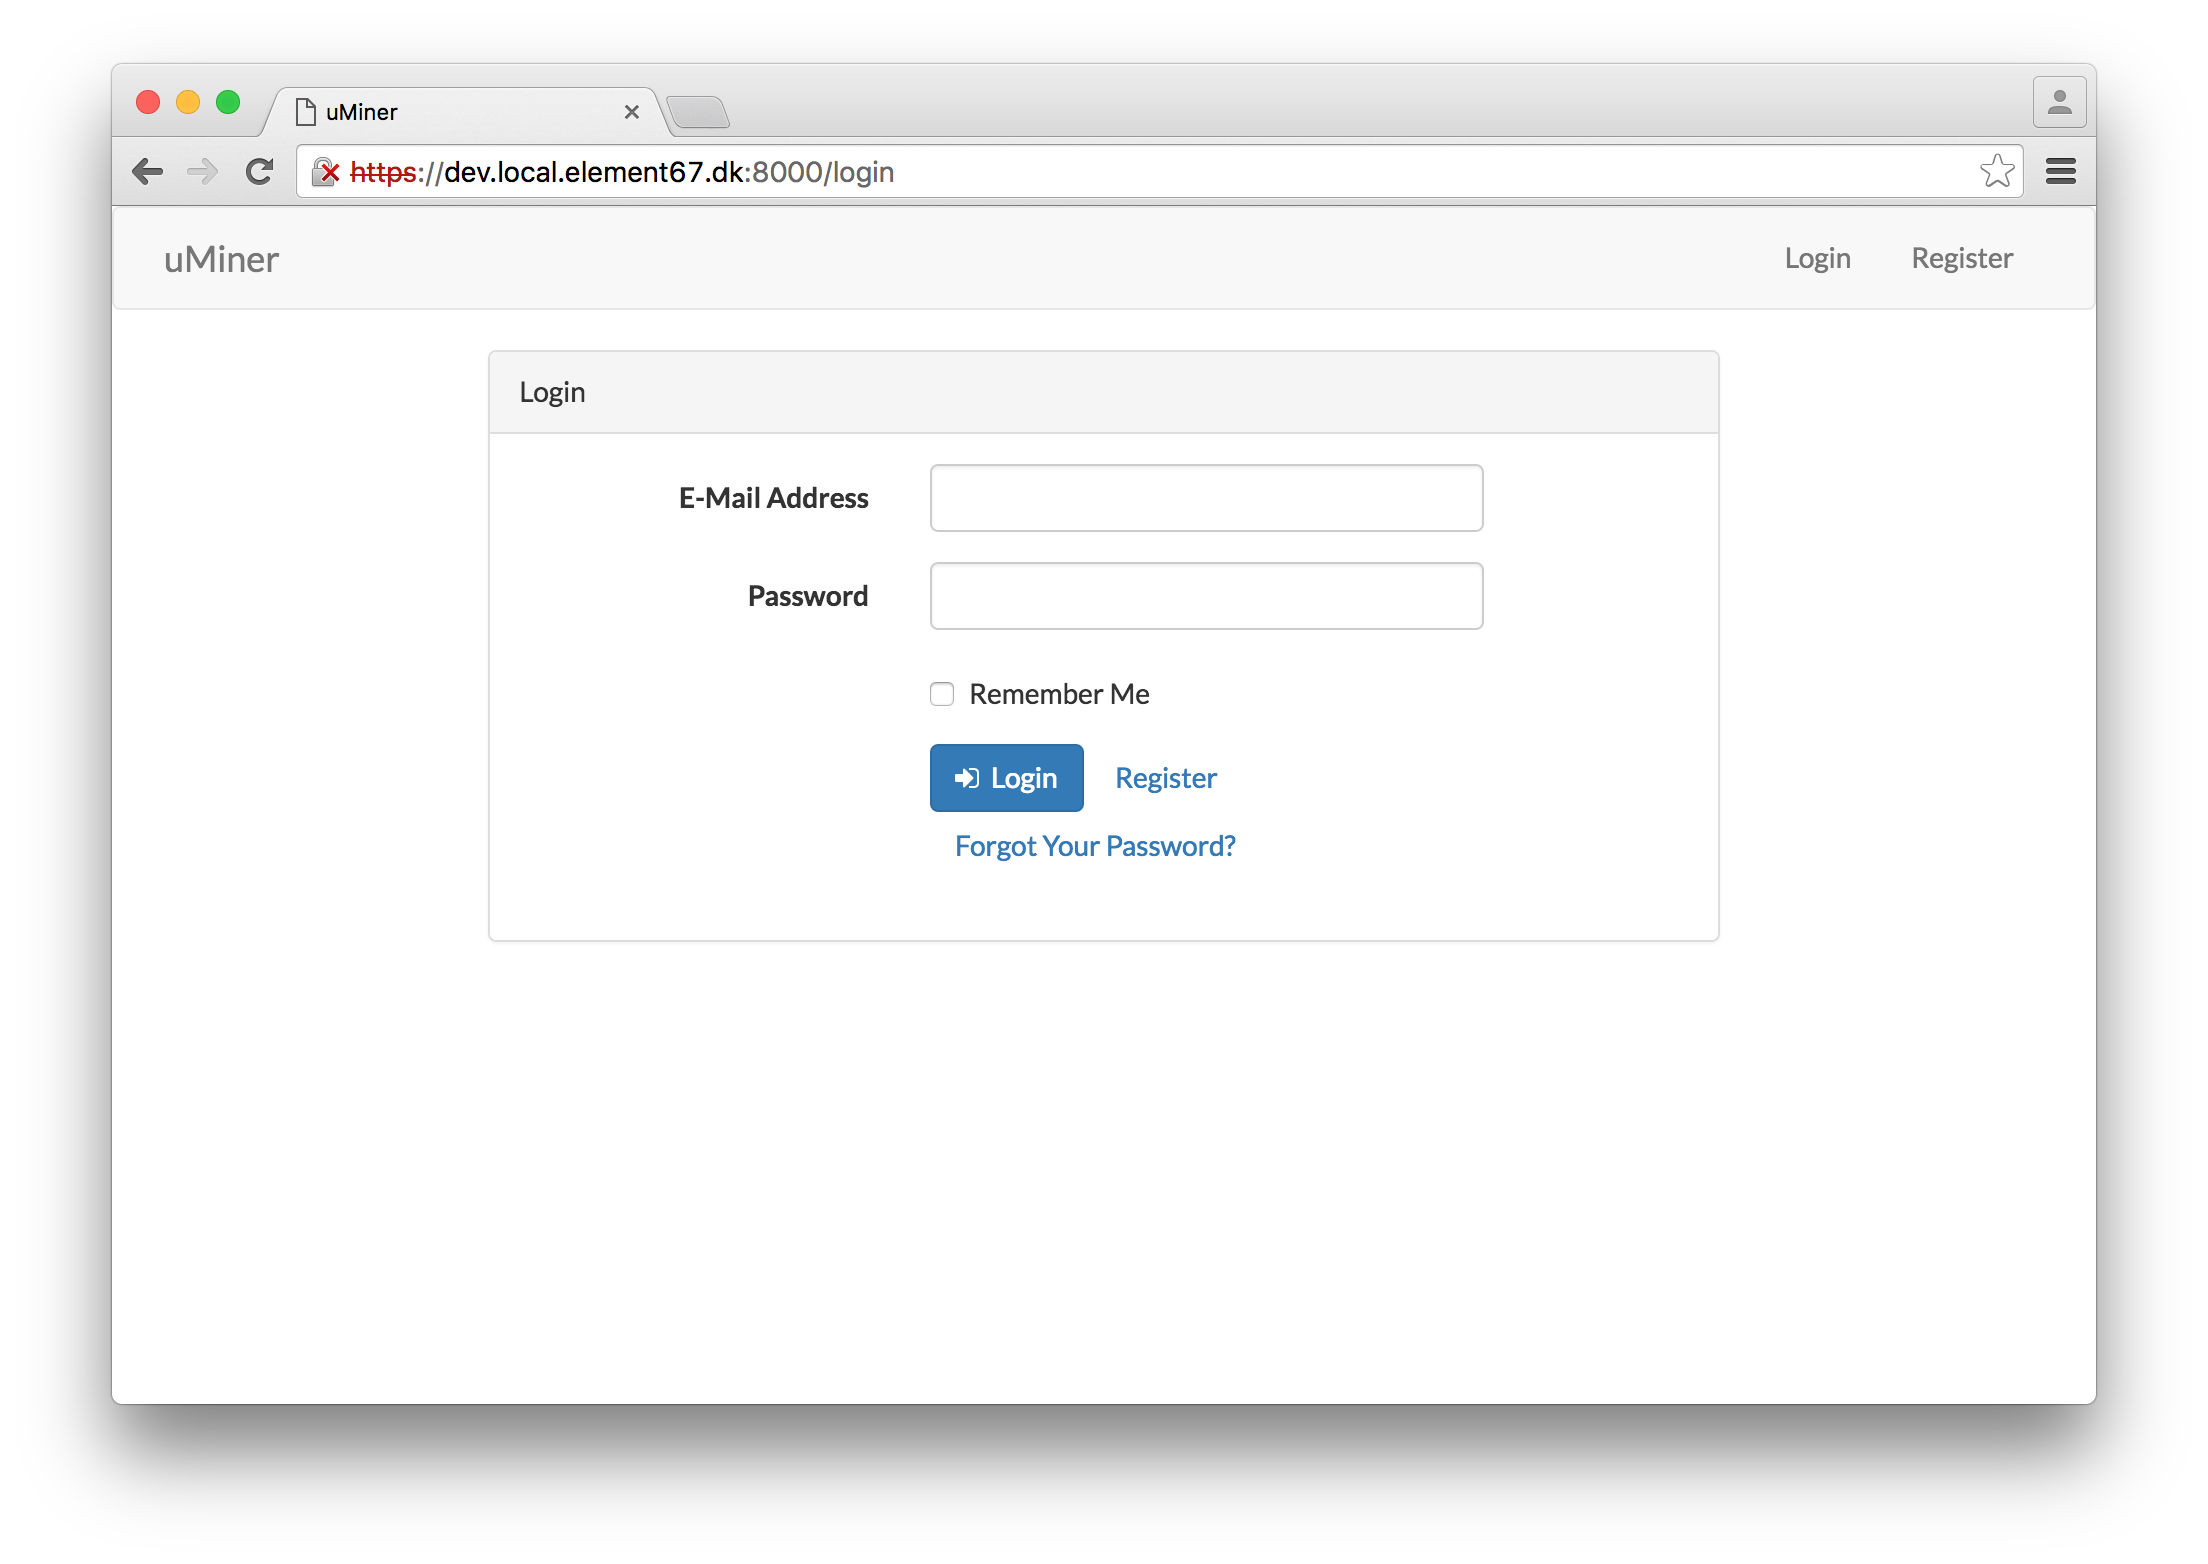
\includegraphics[width=\linewidth]{user_interfaces/web/web_login}
% \caption{Login page.}
% \label{fig:web_login}
% \end{figure}
% \FloatBarrier

\subsection{Creating Campaigns}
\label{sub:creating_campaign}

When a customer is logged in, he has the option to create campaigns. This is done through the site seen in \figref{fig:web_create_campaign}. Here, customers will have to specify different details regarding the campaign. To give customers an ideas of how the participants will view this information, a mobile phone is included on the page, showing the mobile application. Please note that this is only an indication of how it will look, since different phones, with different screen sizes, font settings, etc. will influence the look of the application. A detailed description of all the input fields that the customer must fill out is described below.

\begin{description}
    \item[Campaign title] is used to give participants a rough idea of what the campaign will be used for. This information will visible when participants are browsing campaigns and when viewing details regarding the campaign (as mentioned in \ref{sub:browsing_campaigns}).

    \item[Campaign description] will provide participants with a detailed description of the campaign. This text could possibly contain motivational factory, inclining participants to participate in that specific campaign. This information is only available to participants when viewing the specifications of the campaign (as mentioned in \ref{sub:browsing_campaigns}).

    \item[Campaign author] cannot be specified directly by the customer, but is instead depending on the name of the account that the participant is logged into. Like the campaign title, this information will be included when participants are browsing campaigns and when viewing details regarding the campaign (as mentioned in \ref{sub:browsing_campaigns}).

    \item[Campaign availability] can be specified through the checkbox directly below the description input field. This checkbox is marked by default, making the campaign publicly available, meaning that it is visible for participants when they are browsing the campaigns (as seen in \figref{fig:public_campaigns}). Unchecking this checkbox will cause the campaign to be private, effectively meaning that customers will have to distribute the campaign identifier in order to get participants.

    \item[Sensors] is a section which allows customers to specify which sensors they would like to gather information from. Sensors are divided into four categories, which roughly describes the information that the sensors will collect. In the current implementation participants can join any campaign even though their phone does not have all of the sensors the customer has specified. Customers might be interested in excluding participants who does not have some essential sensors.

    \item[Sample and measurement] consists of five different input fields. The \emph{Snapshots per Campaign} input is used to specify how many snapshots the participant must collect before completing a campaign.

    The \emph{Measurement per Sample}- and \emph{Measurement delay} input fields will change the length of a sample, while the \emph{Samples per Snapshot}- and \emph{Sample delay} input fields will change the length of a Snapshot. Please note that this way of specifying snapshots differs from the internal structure, explained in \secref{sec:modeling_sensor_data}. We did this, since customers might find it easier to specify the delay between measurements and samples, rather than having to calculate the different frequencies.

    The concept of delay, amount of measurements, samples etc. might still be difficult to grasp, so we have included a illustration of a time line. This could possibly aid customers in specifying the different parameters. Ideally, the figure should be responsive, and automatically update whenever customers change the input fields.

    \item[Questionnaire placement] will indicate when participants are prompted with questions. As described previously, in \secref{sub:answering_questionnaired}, this can either be in the beginning, or at the end of a snapshot. We have also had some considerations in regards to when participants should be prompted, which are also described in \secref{sub:answering_questionnaired}.

    \item[Questionnaire] consists of a sequence of questions. Questions can be re-arranged by dragging them up or down in the list. The participants will receive the questions in the order they are presented on this page. If a customer does not specify any question to his/her campaign, the participants will never be prompted to fill out a questionnaire if they have joined that campaign.
\end{description}

% Create campaign
\begin{figure}[!htbp]
\centering
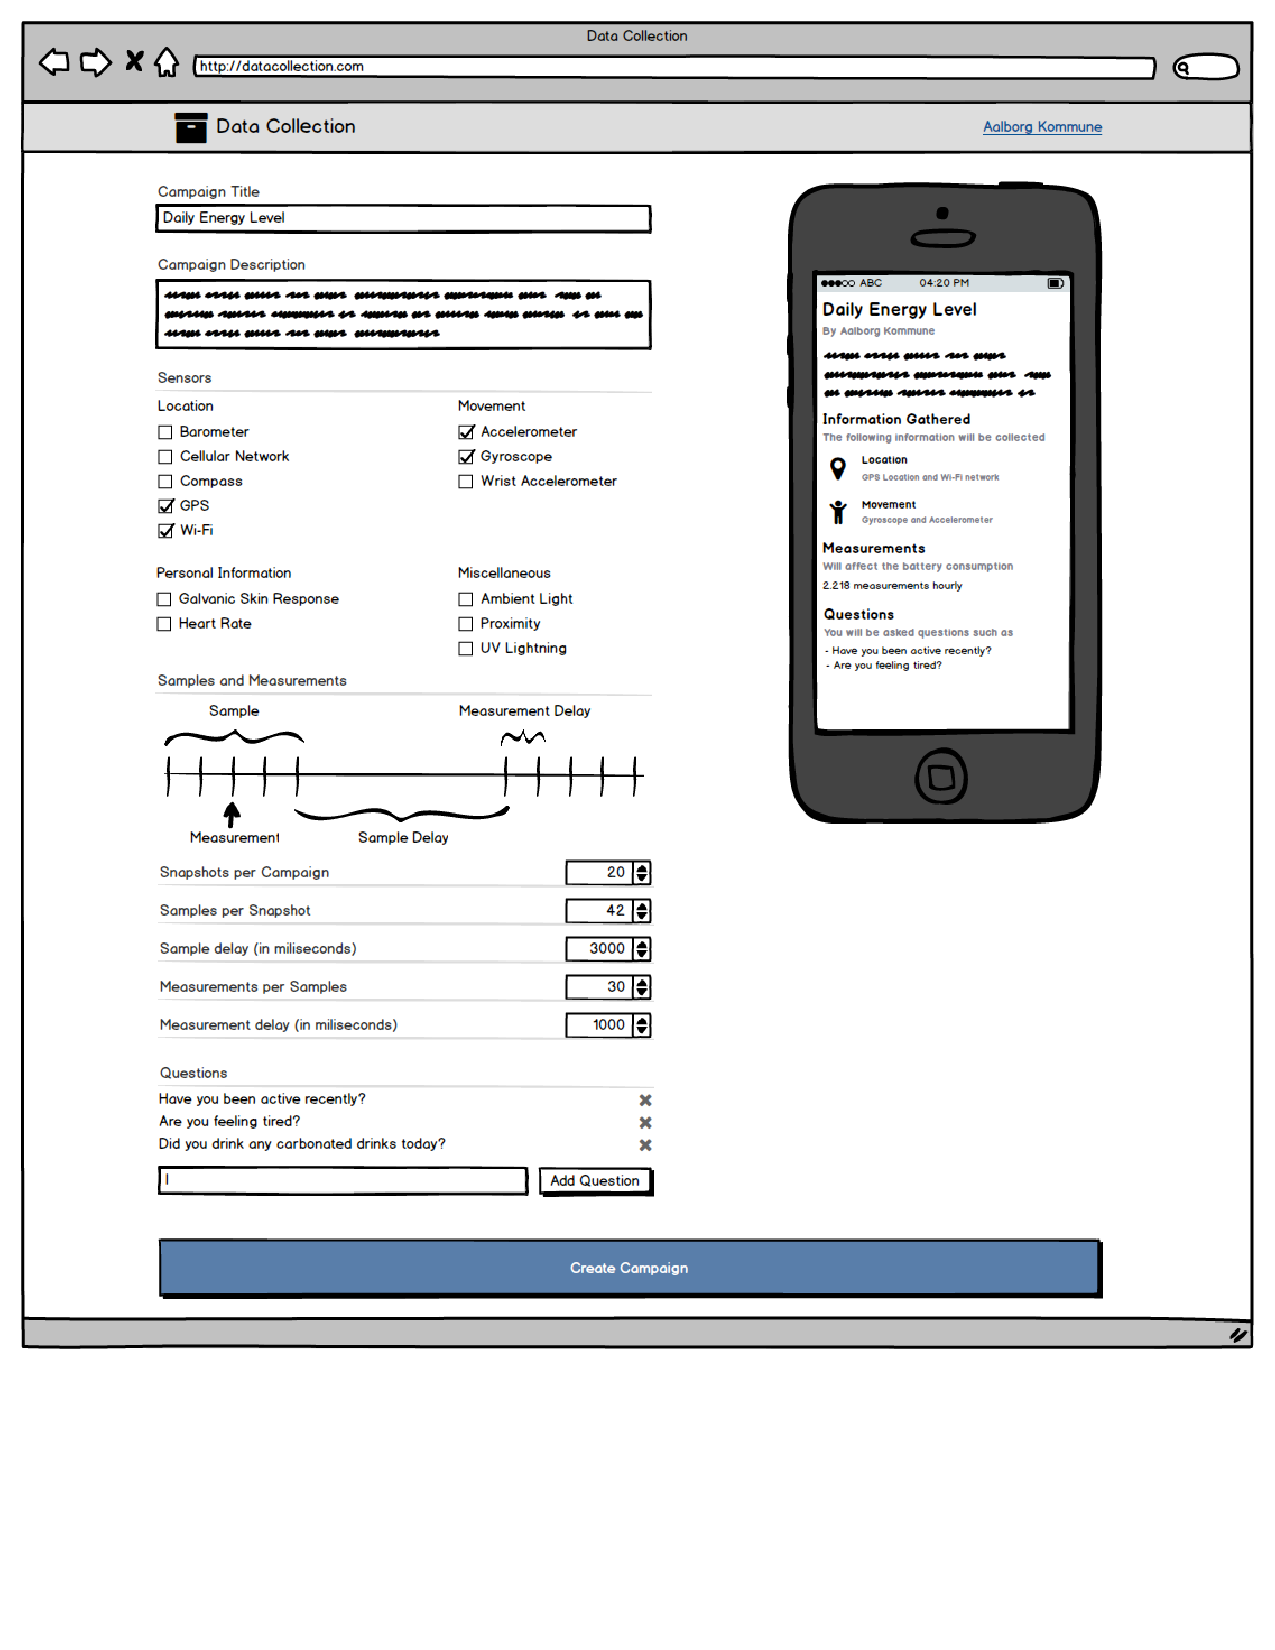
\includegraphics[width=\linewidth]{user_interfaces/web/web_create_campaign}
\caption{Creating Campaigns.}
\label{fig:web_create_campaign}
\end{figure}
\FloatBarrier

\subsection{Viewing Campaign Details and Gathered Snapshots}
\label{sub:viewing_campaign_details}

When customers have created a campaign, it will show up in their list of campaigns, as seen in \figref{fig:web_view_campaigns}. If the customer have not created any campaigns yet, this page will only contain the small description along with the \emph{Create}-button. If the customer presses any of the created campaigns on this page, he will be redirected to a page similar to the one seen in \figref{fig:web_view_campaign}. This page will reflect the values the customer inputted when he created the campaign through the creation page. Furthermore, this page also informs customers regarding the campaign identifier, allowing them to distribute the campaign through other media than our application. On the right side of the page, a \emph{Progress} area has been included. We have included this so customers may get an insight in on how many participants have contributed (\emph{Participants joined}), but also much data has been collected and uploaded to the server (\emph{Snapshots submitted}). One could imagine that it would be possible to extend the system with additional useful metrics, for example displaying the most common time that participants answer questions, which questions makes them close the application, etc.

% View campaigns
\begin{figure}[!htbp]
\centering
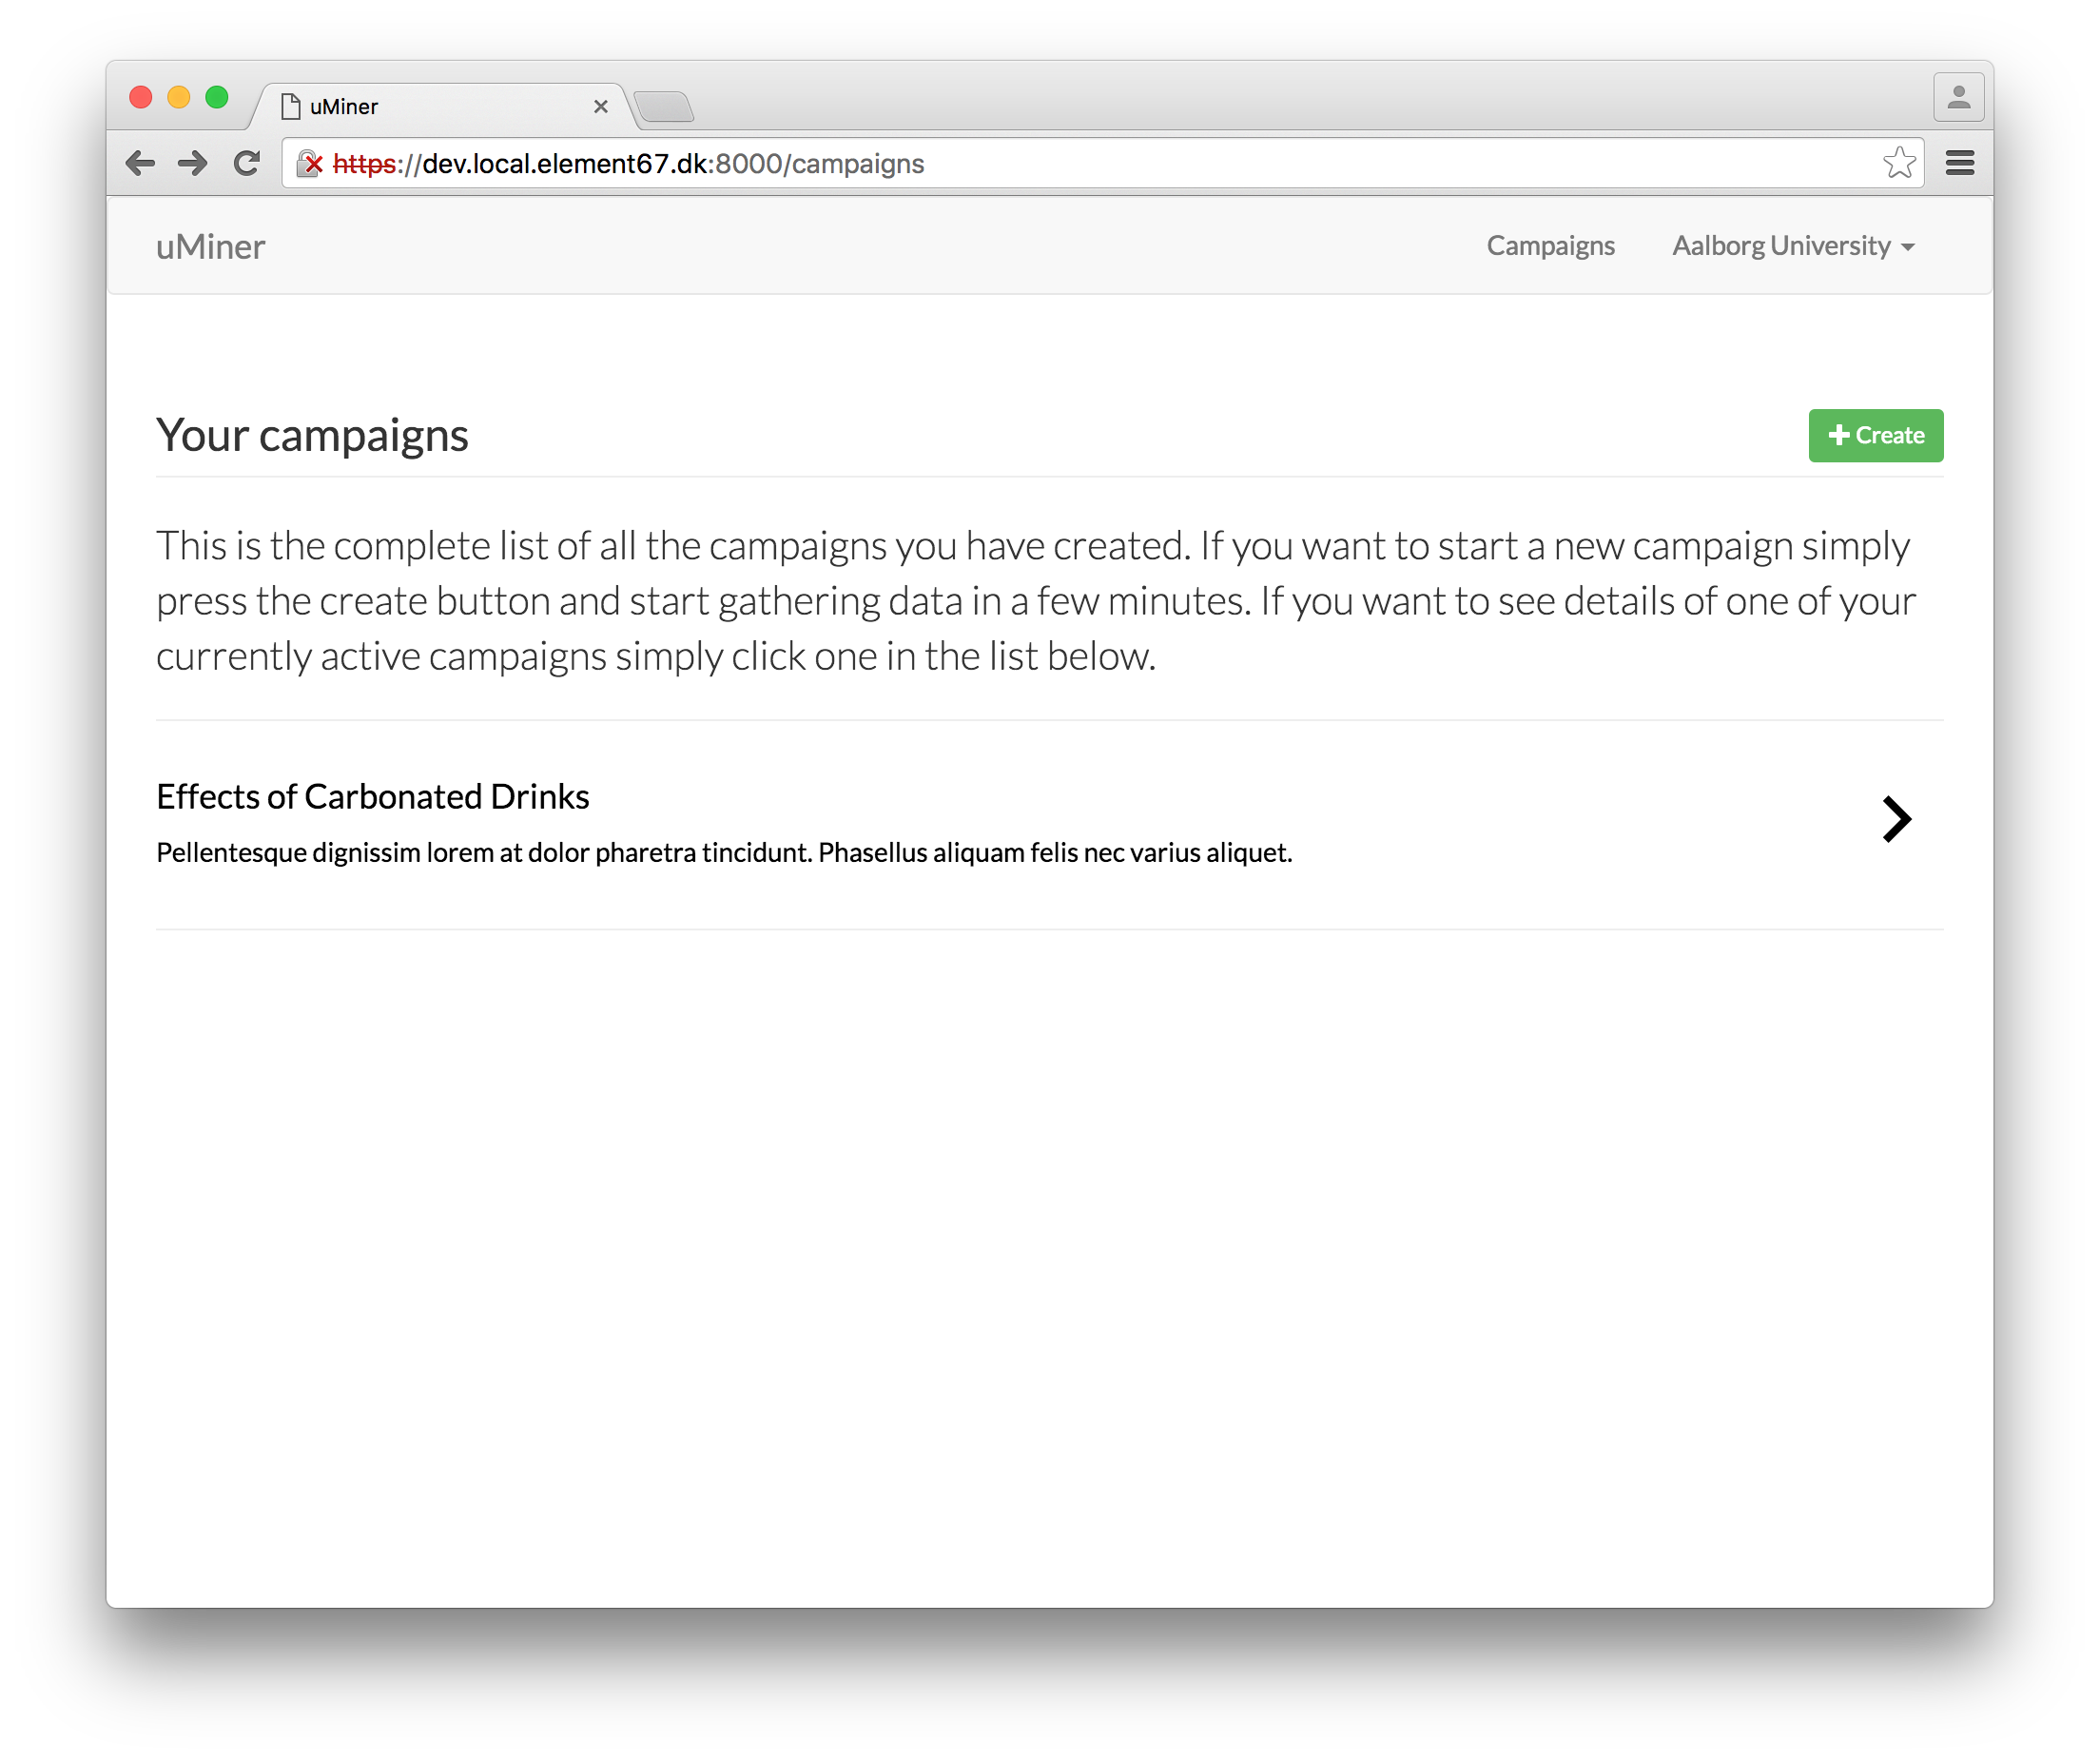
\includegraphics[width=\linewidth]{user_interfaces/web/web_view_campaigns}
\caption{Viewing Campaigns.}
\label{fig:web_view_campaigns}
\end{figure}
\FloatBarrier

% View specific campaign
\begin{figure}[!htbp]
\centering
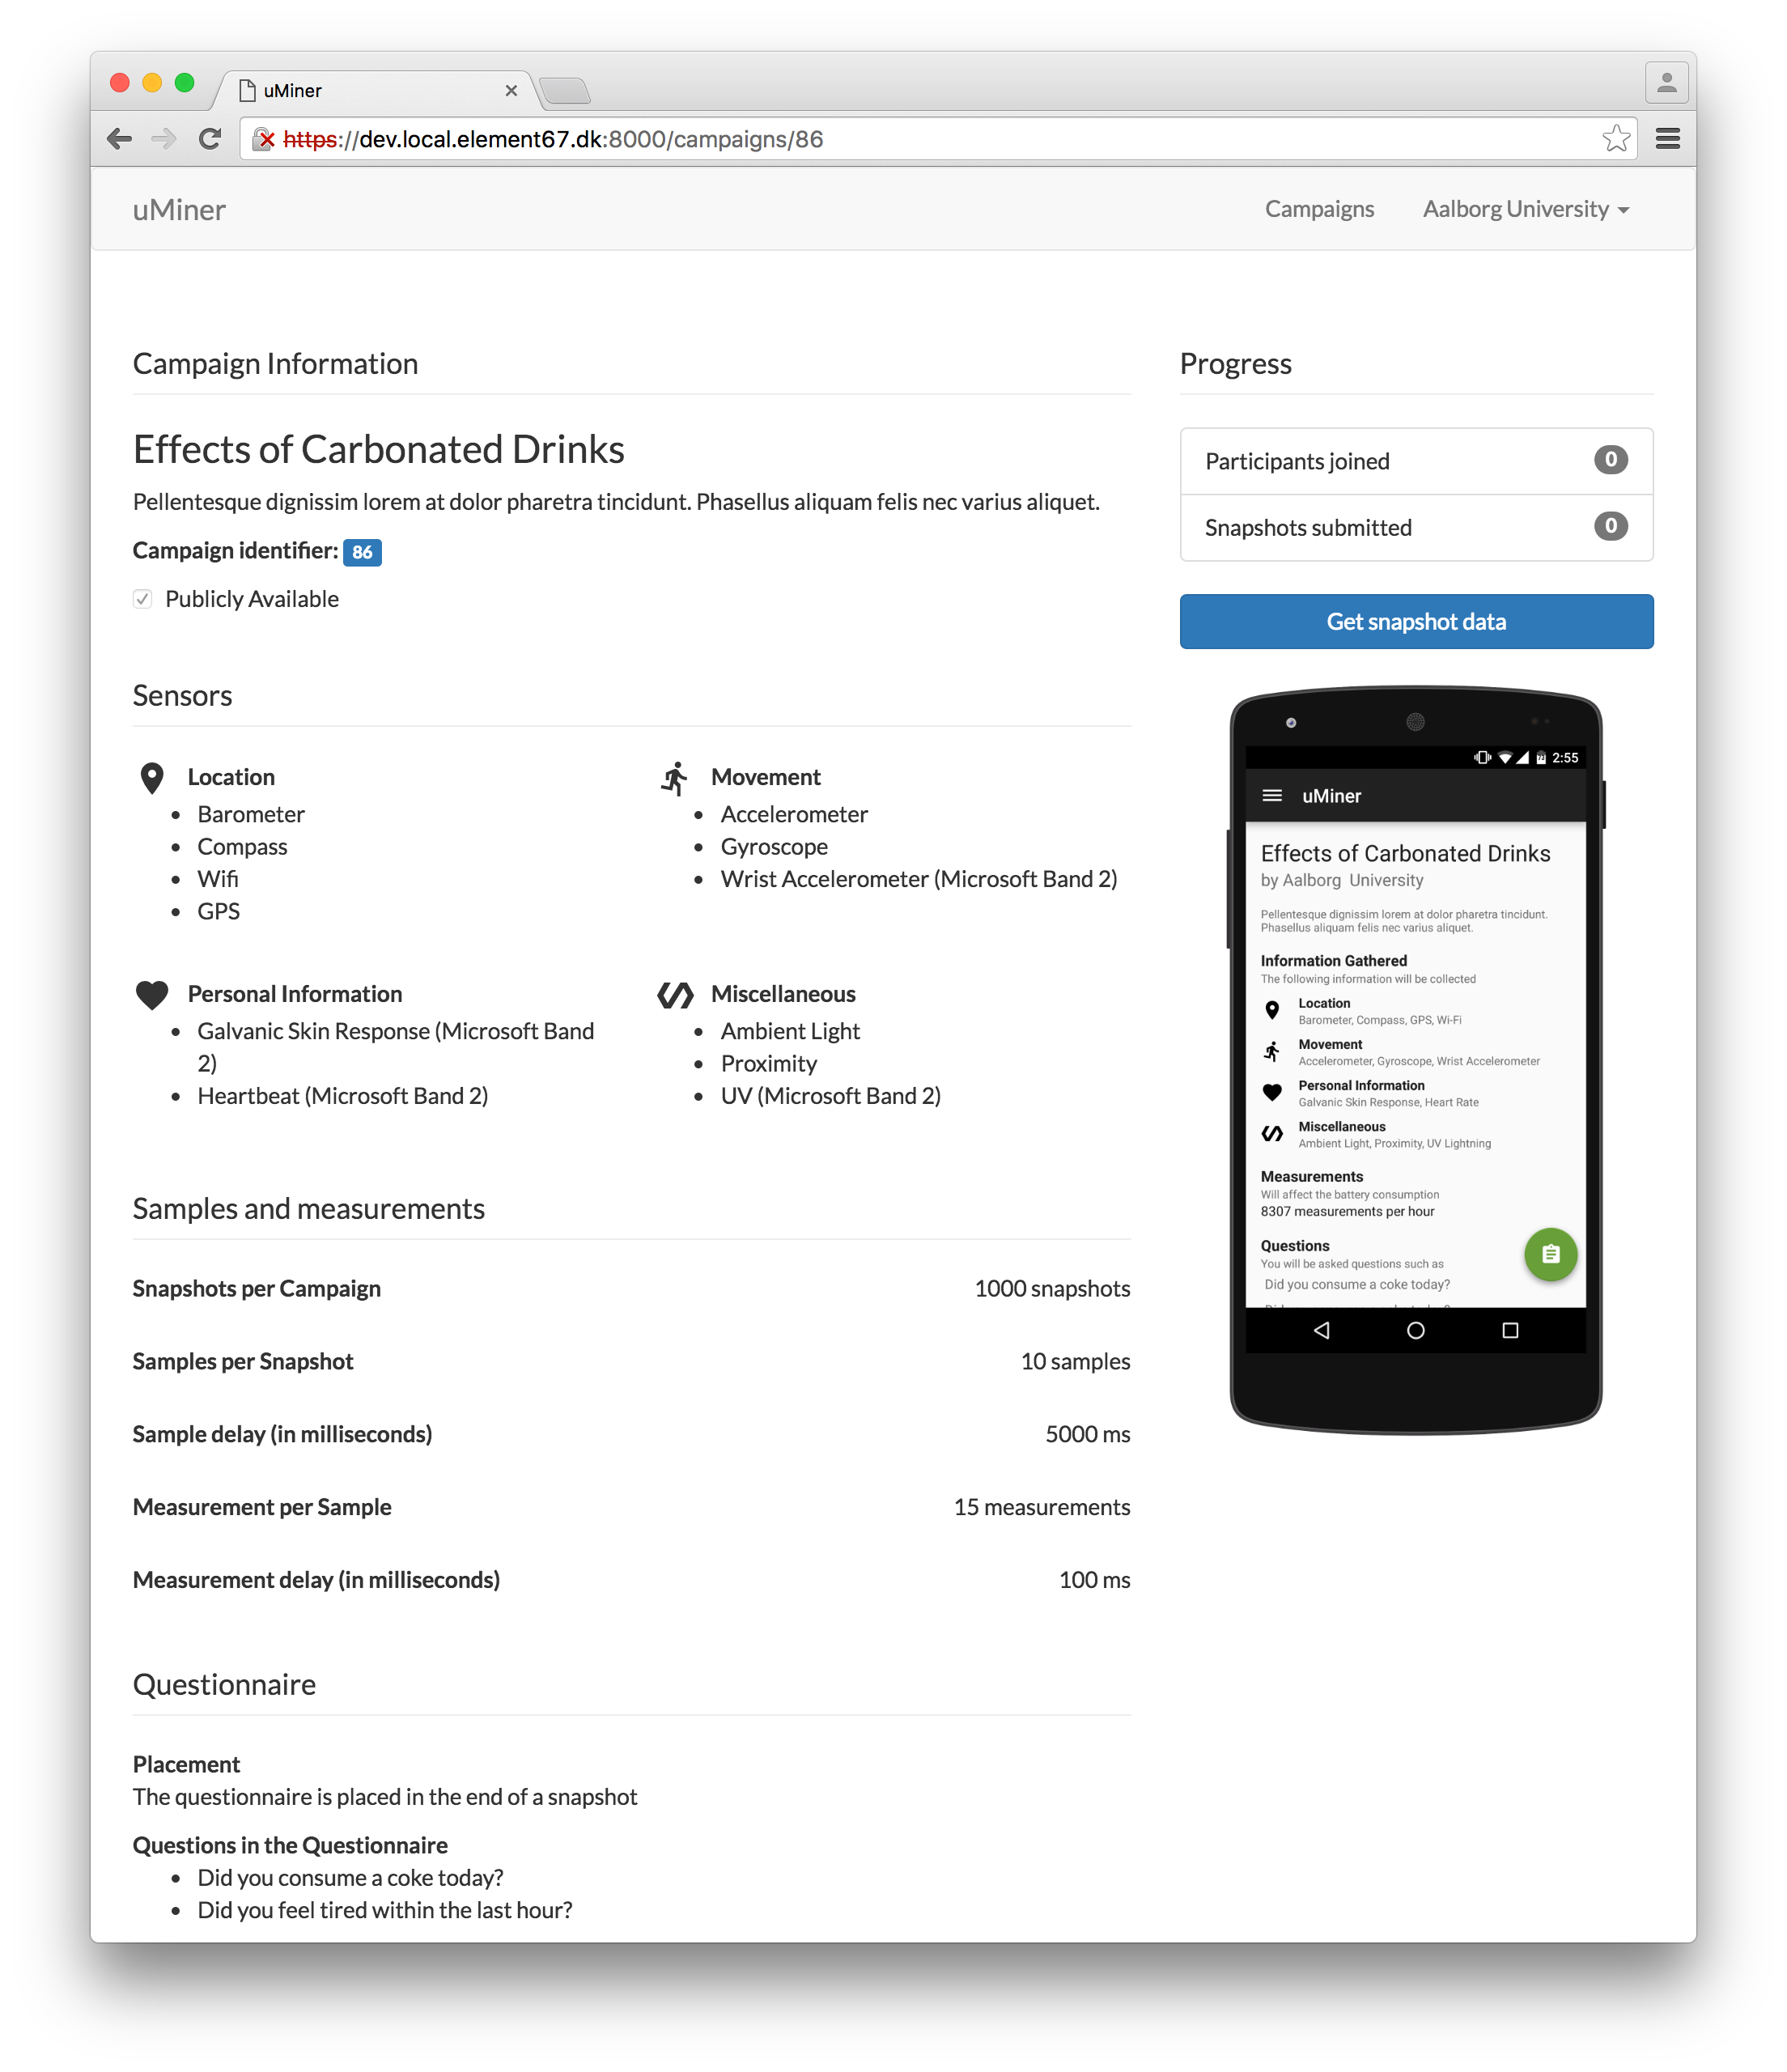
\includegraphics[width=\linewidth]{user_interfaces/web/web_view_campaign}
\caption{Viewing details regarding specific campaign.}
\label{fig:web_view_campaign}
\end{figure}
\FloatBarrier

To view the collected snapshots, submitted by participants, customers can press the \emph{Get snapshot data} button, just below the statistics. This will redirect the user to a site, containing unformatted JSON, describing the different snapshots that have been submitted for that particular campaign. \lstref{lst:snapshot_json_example} shows the structure of the JSON output. The first few entries in the object will describe some meta-information about the snapshots collected, such as the total amount of snapshots collected (\mono{total}). Furthermore, these objects will also describe how to iterate through the data set through pagination, for instance the \mono{per\_page} entry will specify how many snapshots will be displayed per page. To retrieve the next set of snapshots, the customer will have to visit the page specified in the \mono{next\_page\_url} entry. The collected snapshots are stored in the array with the key \mono{data}. A snapshot object also consists of some meta-information, such as who submitted it (\mono{participant\_id}), when it was submitted (\mono{created\_at}) etc. A snapshot furthermore consists of the samples that have been collected, for instance \mono{accelerometerSamples} for samples from the accelerometer sensor. 

\lstinputlisting[
   style = json,
   caption = {Illustration of the JSON structure of collected snapshots.},
   label = {lst:snapshot_json_example},
   float=!htbp,
]{content/user_interface/code_snippets/snapshot_json_example.json}
\FloatBarrier

\subsection{Editing and Deleting Campaigns}
\label{sub:editing_and_deleting_campaigns}

In the current implementation of the system, it is not possible to edit campaigns, since we deemed it to be an unnecessary feature for the project. This decision was based on the fact that there would be no difference in editing the campaign, and deleting and recreate the campaign. A problem with the edit functionality is, if a customer choose to edit a campaign, all the participants who are subscribed to that campaign would have to be notified that the campaign has being edited, and they might not be able to accept the edited campaign, and would have to be forced to unsubscribe from it. Furthermore, all the gathered snapshot would be invalidated, and would need to be removed, or marked as garbage, because there might be missing sensors or labels. It is however possible to implement some different checks, that would inform the participants regarding the updated campaign, asking them to re-subscribe to the campaign. To delete a campaign, customers will have to press the red \emph{Delete} button, which can be seen in \figref{fig:web_view_campaign}. 
\\\\
It is easy to imagine that customers would like to update the title, description, or the questions to correct spelling errors, or give a better clarification of the campaign. This would not require the removal of already collected data, since it would not be invalidated because the semantics of the labels would not change. However, we choose not to pursue any of these editing solutions.
